\documentclass[tikz,border=10pt]{standalone}
\usepackage{tikz}
\usepackage{fontawesome5}
\usetikzlibrary{arrows.meta,positioning,fit,backgrounds,calc,shadows,shapes.geometric,tikzmark}

% Color definitions
\definecolor{lavenderDark}{RGB}{15, 44, 89}
\definecolor{lavenderDeep}{RGB}{10, 28, 58}
\definecolor{lavenderMedium}{RGB}{29, 78, 158}
\definecolor{lavenderLight}{RGB}{240, 246, 255}
\definecolor{lavenderBorder}{RGB}{180, 205, 237}
\definecolor{lavenderAccent}{RGB}{2, 132, 199}
\definecolor{prismNavy}{RGB}{15, 44, 89}
\definecolor{prismBlue}{RGB}{29, 78, 158}
\definecolor{prismTeal}{RGB}{13, 148, 136}
\definecolor{prismMint}{RGB}{236, 253, 245}
\definecolor{prismGold}{RGB}{217, 119, 6}
\definecolor{prismDark}{RGB}{15, 23, 42}
\definecolor{prismSlate}{RGB}{100, 116, 139}

\begin{document}
% Title Slide Decorative Overlay for CiviQ Legal RAG System
\begin{tikzpicture}[x=1cm, y=1cm, font=\sffamily]

  % 1. Top Lavender Banner
  \node[
    rounded corners=5pt,
    fill=lavenderDark,
    drop shadow={shadow xshift=1.5pt, shadow yshift=-2.0pt, opacity=0.35},
    minimum width=15.2cm,
    minimum height=1.05cm,
    inner sep=0pt
  ] at (0, 4.0) {};

  \node[text=white, font=\bfseries\fontsize{11.5}{14}\selectfont] at (0, 4.0) {
    CIVIQ: AI-POWERED LEGAL INFORMATION RETRIEVAL USING RAG
  };

  % 2. College Emblem / Logo Placeholder
  \node[circle, draw=prismSlate, fill=lavenderLight, minimum size=0.95cm, inner sep=0pt] at (0, 2.85) {
    \fontsize{7.5}{9}\selectfont\textbf{\faBalanceScale}
  };

  % 3. Department & College Text
  \node[font=\footnotesize, align=center] at (0, 1.98) {
    \textbf{Dept. of Computer Science \& Engineering}\\[0.12em]
    College of Engineering, Karunagappally
  };

  % 4. Project Group Header
  \node[font=\large\bfseries, text=lavenderDark] at (0, 1.25) {
    B.Tech Project 2026--2027
  };

  % 5. Students & Register Numbers Table
  \node[font=\small] at (0, 0.15) {
    \begin{tabular}{l@{\hspace{2.2cm}}l}
      \textbf{ALEENA ANILKUMAR} & KNP23CS025 \\
      \textbf{ABHINAYA P S}     & KNP23CO007 \\
      \textbf{ADITHYA DINESH}   & KNP23CS016 \\
      \textbf{FATHIMA A}        & KNP23CS047
    \end{tabular}
  };

  % 6. Horizontal Accent Line
  \draw[lavenderDark, line width=0.9pt] (-7.0, -0.85) -- (7.0, -0.85);

  % 7. Project Guide Details
  \node[align=center, font=\footnotesize] at (0, -1.85) {
    {\color{lavenderDark}\textit{Project Guide}}\\[0.25em]
    \textbf{\small Hridhya J}\\[0.12em]
    Assistant Professor\\[0.08em]
    Dept. of Computer Science \& Engineering\\
    College of Engineering, Karunagappally
  };

\end{tikzpicture}
\end{document}
